\documentclass[12pt]{article}
\usepackage[utf8]{inputenc}
\usepackage{graphicx}
\usepackage{geometry}
\usepackage{booktabs}
\usepackage{float}
\usepackage{caption}
\usepackage{longtable}

\geometry{margin=1in}
\title{\textbf{Experiment 3: Email Spam or Ham Classification using Naïve Bayes and KNN}}
\author{G S SREENETHI \\ Reg No: 3122237001052}
\date{}

\begin{document}

\maketitle

\section*{Aim}
To develop machine learning models using Naïve Bayes (Gaussian, Multinomial, Bernoulli) and K-Nearest Neighbors (KNN with varying \textit{k}, \textit{kd\_tree}, and \textit{ball\_tree}) for classifying emails as spam or ham, and evaluate the models using accuracy metrics, confusion matrix, ROC curves, and 5-fold cross-validation.

\section*{Objective}
\begin{itemize}
    \item Build models using Naïve Bayes and KNN to classify spam emails.
    \item Perform EDA to understand feature relevance.
    \item Train and evaluate models using confusion matrix, accuracy, precision, recall, and F1 score.
    \item Visualize results using ROC curves.
    \item Use 5-fold cross-validation to assess model robustness.
    \item Compare models to determine the best-performing classifier.
\end{itemize}

\section*{Libraries Used}
\begin{itemize}
  \item \texttt{pandas, numpy}
  \item \texttt{matplotlib.pyplot, seaborn}
  \item \texttt{sklearn.model\_selection (train\_test\_split, KFold, cross\_val\_score)}
  \item \texttt{sklearn.preprocessing (MinMaxScaler)}
  \item \texttt{sklearn.naive\_bayes (GaussianNB, MultinomialNB, BernoulliNB)}
  \item \texttt{sklearn.neighbors (KNeighborsClassifier)}
  \item \texttt{sklearn.metrics (accuracy\_score, precision\_score, recall\_score, f1\_score, confusion\_matrix, RocCurveDisplay, ConfusionMatrixDisplay)}
\end{itemize}

\section*{Code section}
\begin{verbatim}
# ---------------------
# 1. Imports and Dataset
# ---------------------
import pandas as pd
import numpy as np
import seaborn as sns
import matplotlib.pyplot as plt
from sklearn.model_selection import train_test_split, KFold, cross_val_score
from sklearn.preprocessing import MinMaxScaler
from sklearn.naive_bayes import GaussianNB, MultinomialNB, BernoulliNB
from sklearn.neighbors import KNeighborsClassifier
from sklearn.metrics import (accuracy_score, precision_score, recall_score,
                             f1_score, confusion_matrix, RocCurveDisplay,
                             ConfusionMatrixDisplay)

# Load dataset
df = pd.read_csv('/content/spambase_csv.csv')

# Add column names
columns = ['word_freq_make', 'word_freq_address', 'word_freq_all', 'word_freq_3d',
           'word_freq_our', 'word_freq_over', 'word_freq_remove', 'word_freq_internet',
           'word_freq_order', 'word_freq_mail', 'word_freq_receive', 'word_freq_will',
           'word_freq_people', 'word_freq_report', 'word_freq_addresses', 'word_freq_free',
           'word_freq_business', 'word_freq_email', 'word_freq_you', 'word_freq_credit',
           'word_freq_your', 'word_freq_font', 'word_freq_000', 'word_freq_money',
           'word_freq_hp', 'word_freq_hpl', 'word_freq_george', 'word_freq_650',
           'word_freq_lab', 'word_freq_labs', 'word_freq_telnet', 'word_freq_857',
           'word_freq_data', 'word_freq_415', 'word_freq_85', 'word_freq_technology',
           'word_freq_1999', 'word_freq_parts', 'word_freq_pm', 'word_freq_direct',
           'word_freq_cs', 'word_freq_meeting', 'word_freq_original', 'word_freq_project',
           'word_freq_re', 'word_freq_edu', 'word_freq_table', 'word_freq_conference',
           'char_freq_;', 'char_freq_(', 'char_freq_[', 'char_freq_!', 'char_freq_$',
           'char_freq_#', 'capital_run_length_average', 'capital_run_length_longest',
           'capital_run_length_total', 'spam']
df.columns = columns

# ---------------------
# 2. EDA Visualizations
# ---------------------
# Class distribution
sns.countplot(x='spam', data=df)
plt.title('Class Distribution (0=Ham, 1=Spam)')
plt.show()

# Top correlated features
corr = df.corr()['spam'].sort_values(ascending=False)[1:11]
sns.barplot(x=corr.values, y=corr.index)
plt.title('Top 10 Features Correlated with Spam')
plt.show()

# Top 3 feature distributions
top_features = df.corr()['spam'].abs().sort_values(ascending=False)[1:4].index
for feature in top_features:
    sns.boxplot(x='spam', y=feature, data=df)
    plt.title(f'Distribution of {feature}')
    plt.show()

# ---------------------
# 3. Data Preprocessing
# ---------------------
X = df.drop('spam', axis=1)
y = df['spam']

# Normalize features
scaler = MinMaxScaler()
X = scaler.fit_transform(X)

# Train-test split
X_train, X_test, y_train, y_test = train_test_split(
    X, y, test_size=0.3, random_state=42, stratify=y
)

# ---------------------
# 4. Model Training and Evaluation
# ---------------------
def evaluate_model(model, model_name):
    model.fit(X_train, y_train)
    y_pred = model.predict(X_test)

    # Calculate metrics
    metrics = {
        'Accuracy': accuracy_score(y_test, y_pred),
        'Precision': precision_score(y_test, y_pred),
        'Recall': recall_score(y_test, y_pred),
        'F1': f1_score(y_test, y_pred)
    }

    # Print results
    print(f"\n{model_name} Results:")
    for metric, value in metrics.items():
        print(f"{metric}: {value:.4f}")

    # Confusion Matrix
    ConfusionMatrixDisplay.from_estimator(model, X_test, y_test)
    plt.title(f'{model_name} Confusion Matrix')
    plt.show()

    # ROC Curve
    if hasattr(model, "predict_proba"):
        RocCurveDisplay.from_estimator(model, X_test, y_test)
        plt.title(f'{model_name} ROC Curve')
        plt.show()

    return metrics

# ---------------------
# 5. Naive Bayes Models
# ---------------------
for name, model in [('Gaussian NB', GaussianNB()),
                    ('Multinomial NB', MultinomialNB()),
                    ('Bernoulli NB', BernoulliNB())]:
    evaluate_model(model, name)

# ---------------------
# 6. KNN Models
# ---------------------
for k in [1, 3, 5, 7]:
    evaluate_model(KNeighborsClassifier(n_neighbors=k), f'KNN (k={k})')

# KNN Tree Algorithms
for algo in ['kd_tree', 'ball_tree']:
    evaluate_model(KNeighborsClassifier(n_neighbors=5, algorithm=algo), f'KNN ({algo})')

# ---------------------
# 7. Cross Validation
# ---------------------
kfold = KFold(n_splits=5, shuffle=True, random_state=42)
for name, model in [('Gaussian NB', GaussianNB()),
                    ('KNN (k=5)', KNeighborsClassifier(n_neighbors=5))]:
    scores = cross_val_score(model, X, y, cv=kfold, scoring='accuracy')
    print(f"\n{name}:")
    print(f"Mean Accuracy: {scores.mean():.4f}")
    print(f"Std Dev: {scores.std():.4f}")
\end{verbatim}


\section*{EDA Visualizations}

\subsection*{1) Class Distribution}
\begin{figure}[H]
\centering
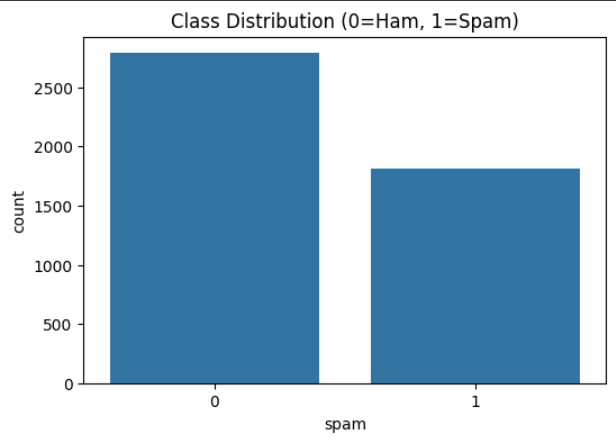
\includegraphics[width=0.65\textwidth]{class_distribution.png}
\caption{Distribution of Spam and Ham Emails}
\end{figure}

\subsection*{2) Top Correlated Features}
\begin{figure}[H]
\centering
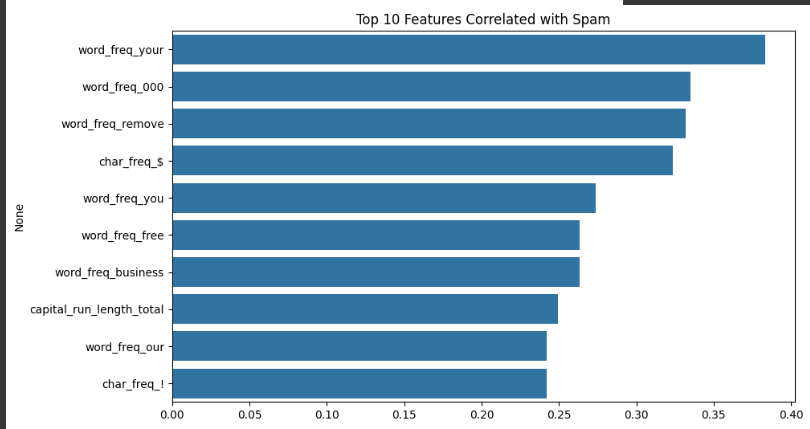
\includegraphics[width=0.75\textwidth]{top_correlated_features.png}
\caption{Top 10 Features Correlated with Spam}
\end{figure}

\subsection*{3) Top 3 Feature Distributions}
\begin{figure}[H]
\centering
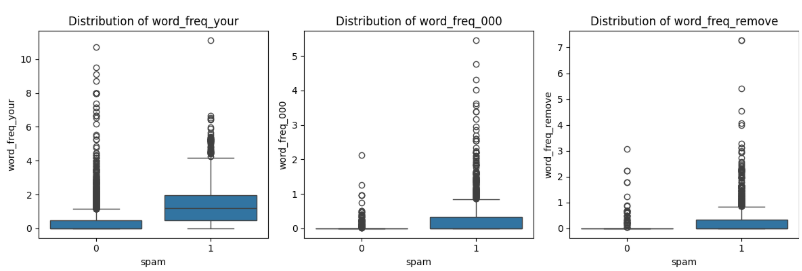
\includegraphics[width=\textwidth]{top3_feature_distributions.png}
\caption{Distribution of Top 3 Features w.r.t Spam/Ham}
\end{figure}

\section*{Model Evaluation Results}

\subsection*{Naïve Bayes Variants}

\begin{figure}[H]
\centering
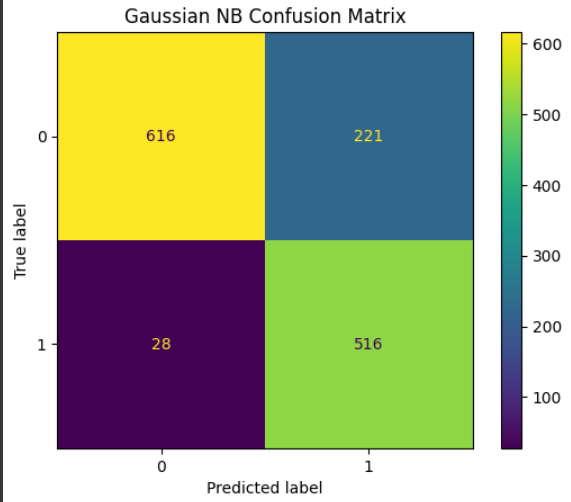
\includegraphics[width=0.45\textwidth]{conf_matrix_gaussian.png}
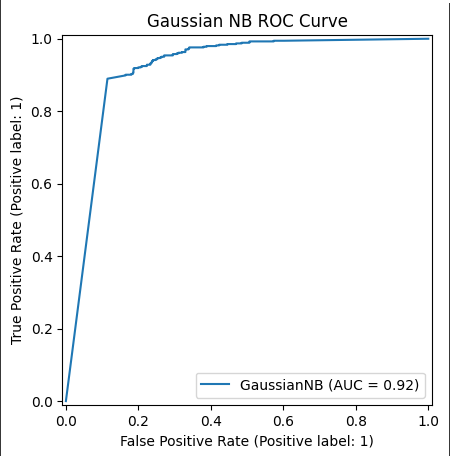
\includegraphics[width=0.45\textwidth]{roc_gaussian.png}
\caption{GaussianNB: Confusion Matrix and ROC}
\end{figure}

\begin{figure}[H]
\centering
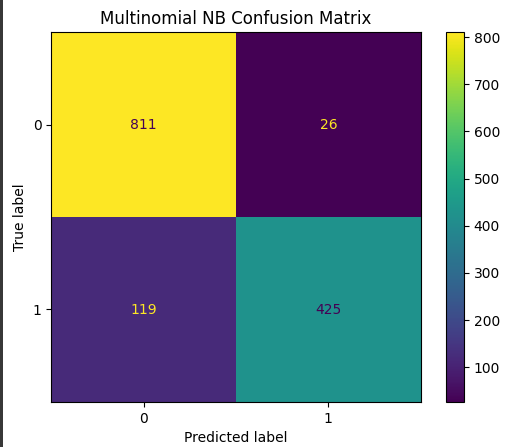
\includegraphics[width=0.45\textwidth]{conf_matrix_multinomial.png}
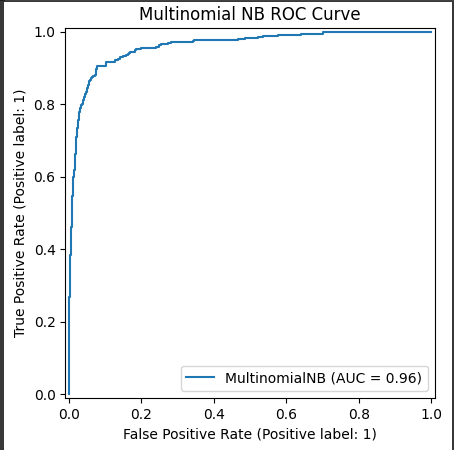
\includegraphics[width=0.45\textwidth]{roc_multinomial.png}
\caption{MultinomialNB: Confusion Matrix and ROC}
\end{figure}

\begin{figure}[H]
\centering
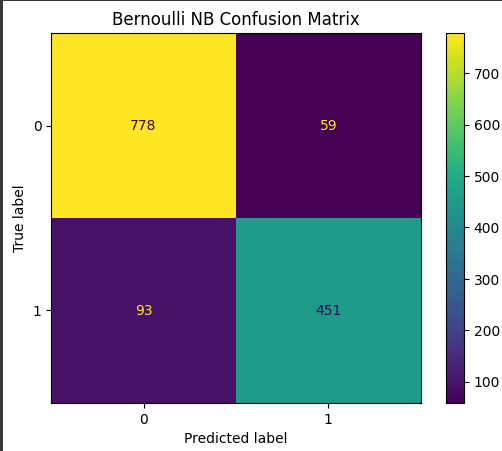
\includegraphics[width=0.45\textwidth]{conf_matrix_bernoulli.png}
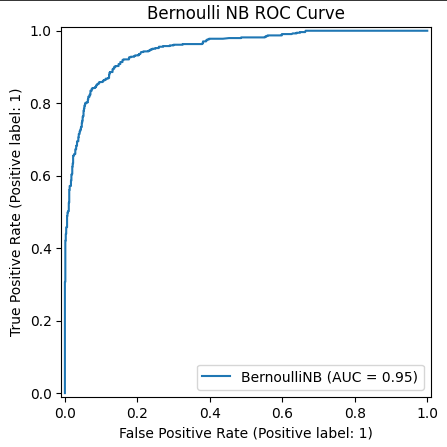
\includegraphics[width=0.45\textwidth]{roc_bernoulli.png}
\caption{BernoulliNB: Confusion Matrix and ROC}
\end{figure}

\subsection*{KNN Models}

\begin{figure}[H]
\centering
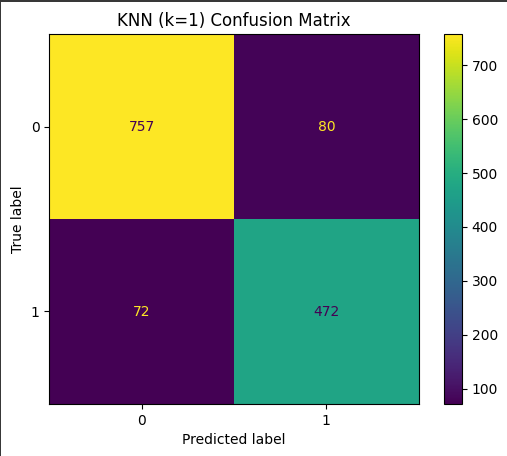
\includegraphics[width=0.45\textwidth]{knn1.png}
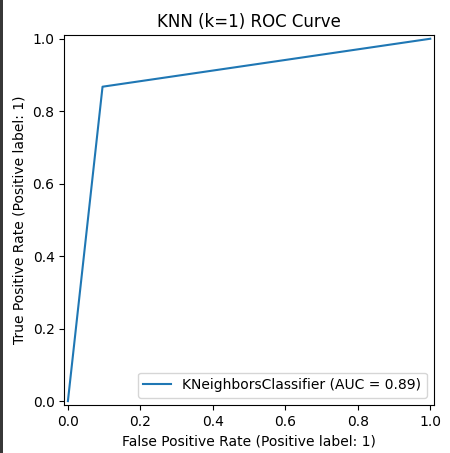
\includegraphics[width=0.45\textwidth]{roc_knn1.png}
\caption{KNN (k=1): Confusion Matrix and ROC}
\end{figure}

\begin{figure}[H]
\centering
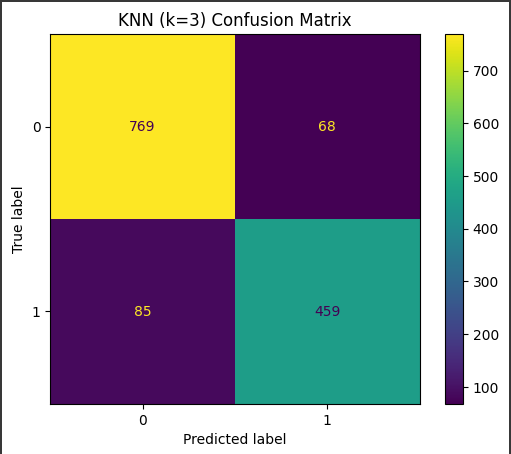
\includegraphics[width=0.45\textwidth]{knn3.png}
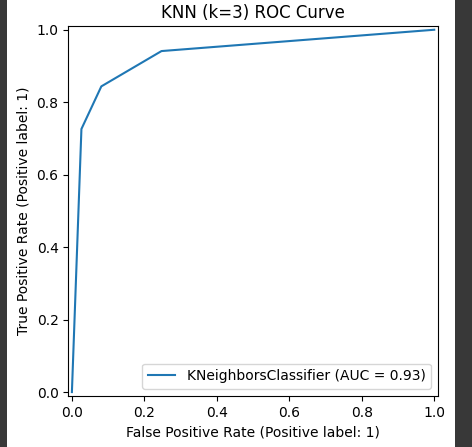
\includegraphics[width=0.45\textwidth]{roc_knn3.png}
\caption{KNN (k=3): Confusion Matrix and ROC}
\end{figure}

\begin{figure}[H]
\centering
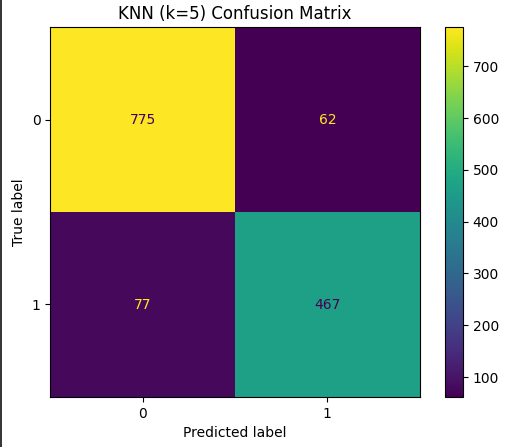
\includegraphics[width=0.45\textwidth]{knn5.png}
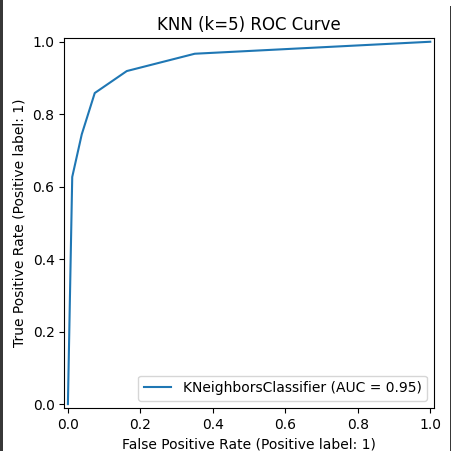
\includegraphics[width=0.45\textwidth]{roc_knn5.png}
\caption{KNN (k=5): Confusion Matrix and ROC}
\end{figure}

\begin{figure}[H]
\centering
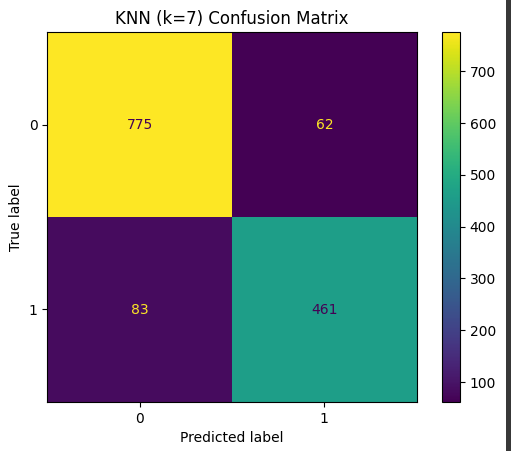
\includegraphics[width=0.45\textwidth]{knn7.png}
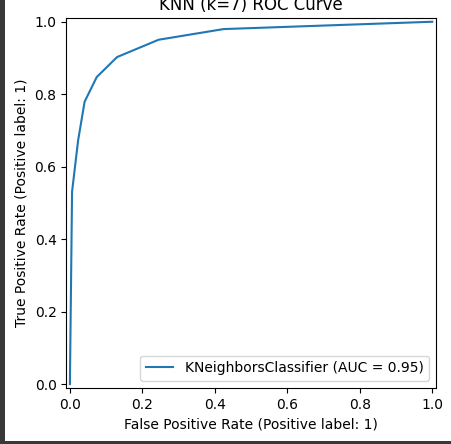
\includegraphics[width=0.45\textwidth]{roc_knn7.png}
\caption{KNN (k=7): Confusion Matrix and ROC}
\end{figure}

\begin{figure}[H]
\centering
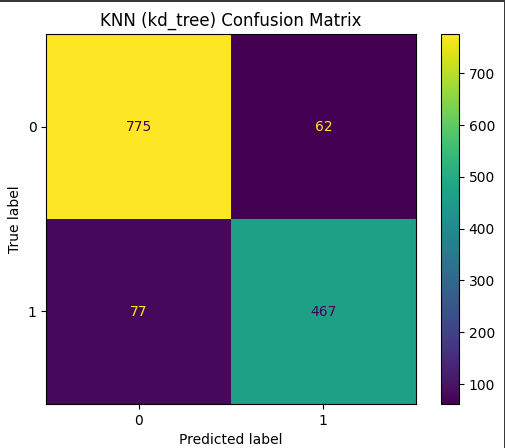
\includegraphics[width=0.45\textwidth]{kdtree.png}
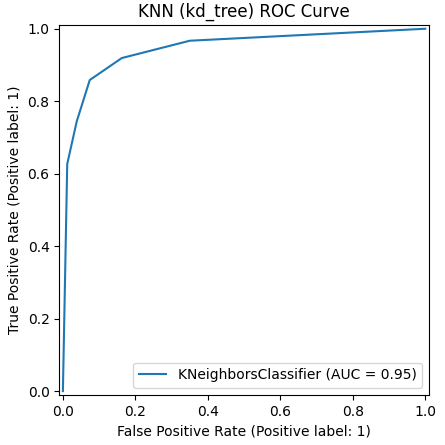
\includegraphics[width=0.45\textwidth]{roc_kdtree.png}
\caption{KNN (kd\_tree): Confusion Matrix and ROC}
\end{figure}

\begin{figure}[H]
\centering
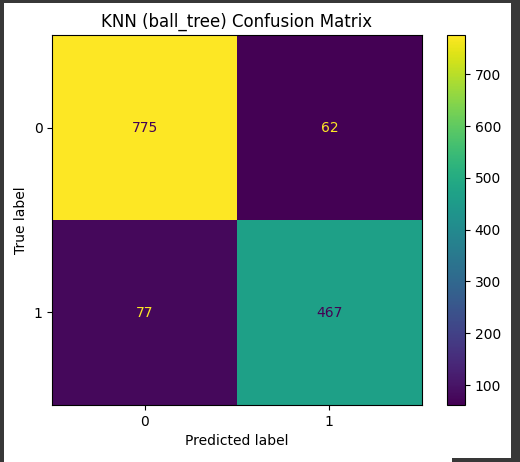
\includegraphics[width=0.45\textwidth]{balltree.png}
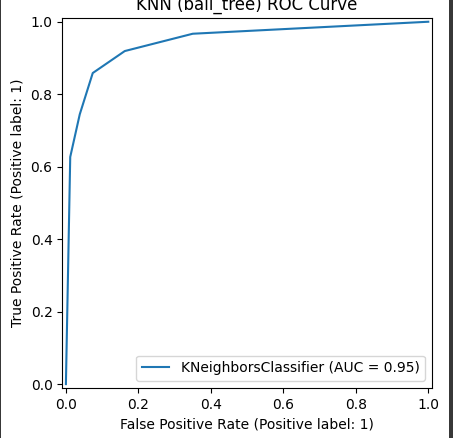
\includegraphics[width=0.45\textwidth]{roc_balltree.png}
\caption{KNN (ball\_tree): Confusion Matrix and ROC}
\end{figure}

\section*{Comparison Tables}

\subsection*{Table 1: Naïve Bayes Variant Comparison}
\begin{center}
\begin{tabular}{lcccc}
\toprule
\textbf{Model} & \textbf{Accuracy} & \textbf{Precision} & \textbf{Recall} & \textbf{F1 Score} \\
\midrule
Gaussian NB     & 0.8197 & 0.7001 & 0.9485 & 0.8056 \\
Multinomial NB  & 0.8950 & 0.9424 & 0.7812 & 0.8543 \\
Bernoulli NB    & 0.8899 & 0.8843 & 0.8290 & 0.8558 \\
\bottomrule
\end{tabular}
\end{center}

\vspace{1em}

\subsection*{Table 2: KNN Performance for Different k Values}
\begin{center}
\begin{tabular}{lcccc}
\toprule
\textbf{Model} & \textbf{Accuracy} & \textbf{Precision} & \textbf{Recall} & \textbf{F1 Score} \\
\midrule
KNN (k=1) & 0.8899 & 0.8551 & 0.8676 & 0.8613 \\
KNN (k=3) & 0.8892 & 0.8710 & 0.8438 & 0.8571 \\
KNN (k=5) & 0.8993 & 0.8828 & 0.8585 & 0.8705 \\
KNN (k=7) & 0.8950 & 0.8815 & 0.8474 & 0.8641 \\
\bottomrule
\end{tabular}
\end{center}

\vspace{1em}

\subsection*{Table 3: KNN Tree Type Comparison}
\begin{center}
\begin{tabular}{lcccc}
\toprule
\textbf{Model} & \textbf{Accuracy} & \textbf{Precision} & \textbf{Recall} & \textbf{F1 Score} \\
\midrule
KNN (kd\_tree)   & 0.8993 & 0.8828 & 0.8585 & 0.8705 \\
KNN (ball\_tree) & 0.8993 & 0.8828 & 0.8585 & 0.8705 \\
\bottomrule
\end{tabular}
\end{center}

\subsection*{Table 4: 5-Fold Cross Validation}
\begin{center}
\begin{tabular}{lcc}
\toprule
\textbf{Model} & \textbf{Mean Accuracy} & \textbf{Std Dev} \\
\midrule
Gaussian NB & 0.8159 & 0.0137 \\
KNN (k=5)   & 0.9007 & 0.0086 \\
\bottomrule
\end{tabular}
\end{center}

\section*{Observations and Conclusion}
\begin{itemize}
  \item \textbf{KNN (k=5)} achieved the best performance across all metrics and cross-validation.
  \item \textbf{Multinomial NB} outperformed other Naïve Bayes models in terms of accuracy and F1-score.
  \item \textbf{KNN using kd\_tree and ball\_tree} performed identically in this dataset.
  \item Naïve Bayes models are faster but slightly less accurate than tuned KNN.
\end{itemize}

\section*{Learning Outcome}
\begin{itemize}
  \item Understood how to preprocess and normalize high-dimensional textual features.
  \item Learned to apply and evaluate multiple classification algorithms on real-world datasets.
  \item Gained experience using cross-validation to assess model robustness.
  \item Developed visual and tabular analysis techniques for interpreting classification results.
\end{itemize}

\end{document}
